%\documentclass[t,handout]{beamer}
\documentclass{beamer}


\usepackage[utf8]{inputenc}
\usepackage[portuguese]{babel}
\usepackage[tight]{subfigure}
\usepackage{graphicx}
\usepackage{color}
\usepackage{url}
% \usepackage{listings}
%\usepackage[alf]{abntcite}

%Pacote de listagem de c�digo
\usepackage{listings}
\lstset{numbers=left, stepnumber=1, firstnumber=1,
numberstyle=\tiny, extendedchars=true, breaklines=true, frame=tb,
basicstyle=\footnotesize, stringstyle=\ttfamily,
showstringspaces=false }


%\usetheme{Frankfurt} %LEGAL     !!!
% \usetheme{Madrid}     %LEGAL/L%IMPO/COM CAIXA     (sem barra de desenvolvimento)

% \usetheme{Antibes} %NAO
%\usetheme{Berlin} %PODE SER...     (BARRA DE DESENVOLVIMANTO)
% \usetheme{Berkeley}     %FEIO
% \usetheme{Boadilla} %TUDO BRANCO...
% \usetheme{Copenhagen}     %NAO
% \usetheme{Darmstadt} %LEGAL!     !!!
 \usetheme{Dresden}     %LEGAL/LIMPO/SEM CAIXA     (sem caixa fica ruim...)

% \usetheme{Goettingen}     %FEIO DEMAIS!
%\usetheme{Ilmenau} %LEGAL (forte candidato)
% \usetheme{JuanLesPins} %BACANA
% \usetheme{Luebeck}     %FEIO

% \usetheme{Malmoe}     %FEIO
% \usetheme{Warsaw} %NAO...
% \usetheme{Seattle}
% \usetheme{CambridgeUS}
% \usetheme{Singapore}

% \usecolortheme[RGB={130,35,150}]{structure}
% \usecolortheme[RGB={33,33,94}]{structure}
\usecolortheme[RGB={134,153,188}]{structure}
\setbeamertemplate{footline}[frame number]
\setbeamertemplate{navigation symbols}{}

%Hide subsections on teable of contents
%\hypersetup{bookmarksopen=true,bookmarksopenlevel=4}
%\setcounter{tocdepth}{2}



\author[L. Medeiros]{Aluno: Leonardo Melo de Medeiros}
\date{\today}
\institute[]{Orientador: Leandro Dias da Silva\\
						 Orientador: Hyggo Oliveira de Almeida \\ 
						 Universidade Federal de Campina Grande - UFCG}
\title{Uma Abordagem de Monitoramento dos Sinais Motores da Doença de Parkinson Baseada em Jogos Eletrônicos}
%\logo{
\includegraphics[width=0.2\linewidth]{img/logo.png}}
\subtitle{Defesa de Tese}

\begin{document}

\begin{frame}
  \titlepage
\end{frame}

% \section{Roteiro}
% \AtBeginSection[]
{\frame{
\frametitle{Roteiro}
%\tableofcontents
\tableofcontents[hideallsubsections]
}
}





\section{Introdução}
\subsection{Motivação}

\begin{frame}{Sistemas de Monitoramento de Saúde}
  \begin{block}{}
  \center
      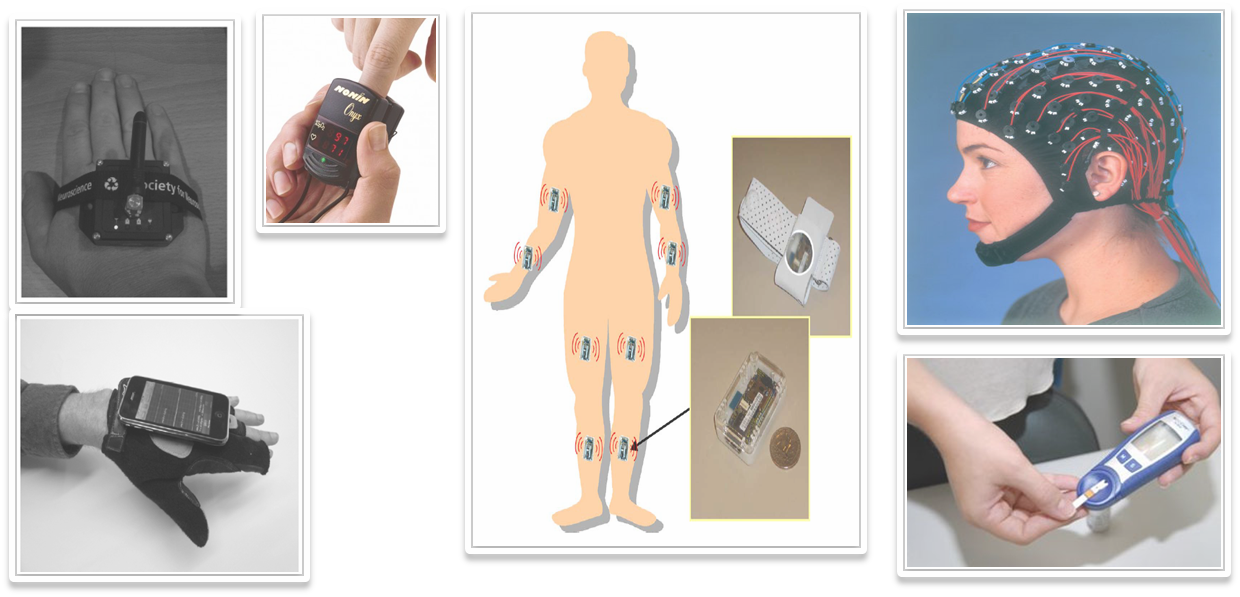
\includegraphics[height=1.8 in]{img/sismonsaude.png}
  \end{block}
  \begin{block}{}  
  A concepção de um sistema não invasivo de monitoramento é um grande desafio~\cite{alemdar2015}.
  \end{block}
\end{frame}




\begin{frame}{Aplicações dos Sistemas de Monitoramento da Saúde (SMS)}  
  \begin{block}{}
  Atualmente, os Sistemas de Monitoramento da Saúde (SMS) permitem ao médico:
  \begin{itemize}[<+->]
   \item Tratar preventivamente e pró-ativamente o estado de saúde~\cite{healthmonitoring2013}; 
   \item Reabilitar o paciente~\cite{sacbespoke2014};
   \item Melhorar a qualidade de vida~\cite{sacsvmhms2014}. 
  \end{itemize} 
  \end{block} 
\end{frame}


\begin{frame}{Estratégias de Monitoramento da Saúde}
  \begin{block}{}
      \center 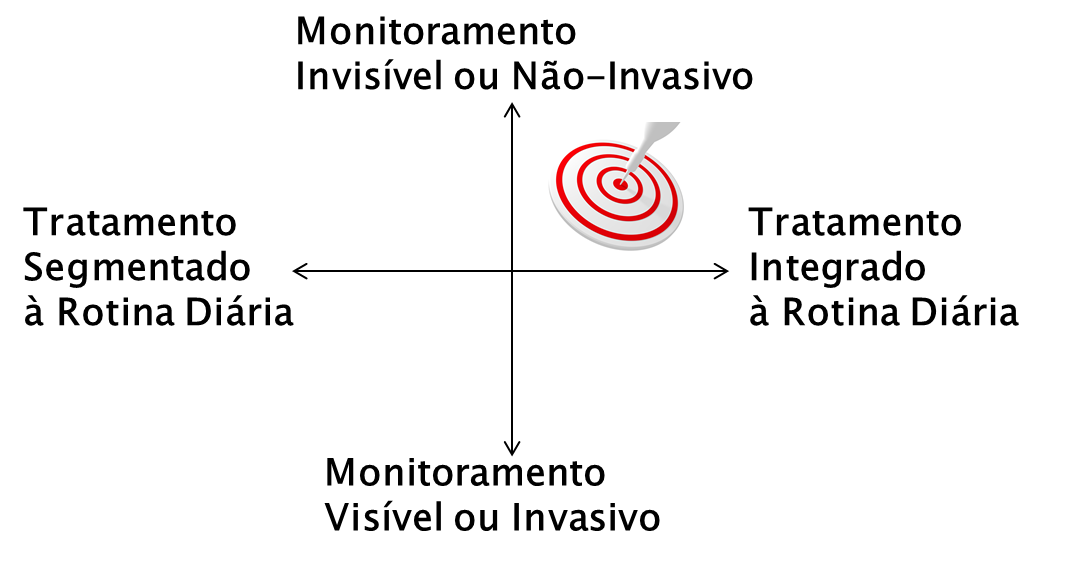
\includegraphics[height=2.2 in]{img/estrategmonitorament.png}
  \end{block}
%   \begin{block}{}
% As tecnologias de monitoramento para serem aceitas precisam preservar a privacidade do usuário e integrar-se à sua rotina diária~\cite{alemdar2015}.
%   \end{block}
\end{frame}


\begin{frame}{SMS da Saúde Motora}  
  \begin{block}{}  
  Atualmente, os SMS da saúde motora permitem:  
    \begin{itemize}[<+->]
    \item quantificar as habilidades motoras dos usuários~\cite{manumeterjbhi2014,patel_monitoring_2009};
    \item analisar a marcha dos usuários~\cite{robotgait2014}
    \item identificar sinais de bradicinesia (lentidão dos movimentos) presente no Parkinson~\cite{ambulatoryparkinson2010}. 
    \end{itemize}   
  \end{block}   
\end{frame}

\begin{frame}{Abordagem Proposta}
  \begin{block}{}
      \center 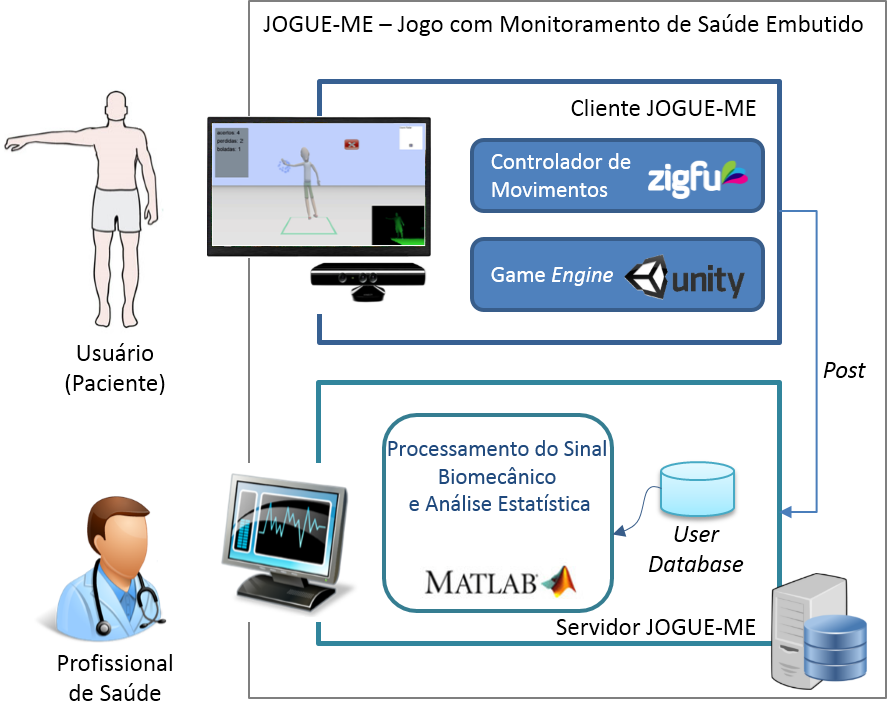
\includegraphics[height=1.8 in]{img/visaosistema.png}
  \end{block}
  \begin{block}{ }
Nesta Tese, propomos monitorar a saúde de uma forma não invasiva usando jogos eletrônicos. 
  \end{block}
\end{frame}


\subsection{Jogos Para Saúde}
\begin{frame}{Jogos Aplicados à Saúde}
	\begin{block}{}	
	Nos últimos anos, houve o surgimento de jogos para apoiar a prática de atividade física. Como por exemplo:
	
	\begin{itemize}[<+->]
	    \item Melhoria da saúde do idoso com: visado a reabilitação motora dos idosos~\cite{sacbespoke2014};
	    \item Jogos com sensores hápticos para quantificar a habilidade motora do paciente com Parkinson ~\cite{atkinson2010};
	    \item Jogos para o monitoramento dos sinais vitais(Batimento cardíaco)~\cite{Sinclair:2009:UVB:1515604.1515617}.
	\end{itemize}
	\end{block}
\end{frame}


\begin{frame}{Motivação para uso de jogos para monitoramento dos dados motores}
	\begin{block}{}
	\begin{itemize}[<+->]
	    \item Percentual expressivo de adultos e idosos que usam jogos em sua rotina diária (27\% acima dos 50 anos~\cite{esa2015});
	    \item As tecnologias de sensores de movimento presentes nos jogos eletrônicos;
	    \item Reprodução de movimentos específicos em um ambiente lúdico.
	\end{itemize}
	\end{block}
	
	\begin{alertblock}{}<4->
	Monitorar os sinais em permite um melhor gerenciamento da doença e, por consequência, uma melhora na qualidade de vida.
	\end{alertblock}
\end{frame}


\begin{frame}{Objetivo Principal}
  \begin{block}{}
  Conceber um SMS embutido num jogo eletrônico para motivar e abstrair o monitoramento dos sinais motores de uma maneira não invasiva.
  \end{block}
\end{frame}


\begin{frame}{Etapas do Trabalho}
	\begin{block}{}
	  A da metodologia deste trabalho consistiu de três etapas sequenciais:
		  \begin{description}[<+->]
		  \item[ETAPA 1] Quais os benefícios de acompanhar os sinais motores do paciente diariamente, do ponto de vista do profissional da saúde?
		  \item[ETAPA 2] Como melhor adquirir e quantificar sinais motores utilizando sensores de movimento para monitorar os sinais do Parkinson?
		  \item[ETAPA 3] Na perspectiva dos usuários, a abordagem de quantificar os sinais motores é considerada não-invasiva e aplicável à rotina diária?
		  \end{description}
	\end{block}
\end{frame}

\section{Estudo de Caso}
\subsection{Parkinson}
\begin{frame}{Estudo de Caso}
  \begin{block}{Doença de Parkinson}
   Como estudo de caso, escolhemos Parkinson por ser uma doença neurodegenerativa crônica, progressiva e com causa desconhecida. 
   \begin{itemize}
    \item Comum em idosos;
    \item Existem casos precoces em indivíduos antes dos 40 anos.
   \end{itemize}
  \end{block}
\end{frame}


\begin{frame}{Doença de Parkinson (Parkinson)}
  \begin{block}{}
    O Parkinson é uma afecção do sistema nervoso central, a qual é expressa de forma crônica e progressiva. 
      \begin{itemize}[<+->]
       \item Causada pela morte dos neurônios produtores de dopamina da substância negra ~\cite{protpar010}. 
       \item Caracterizada pelos sinais cardinais de rigidez, bradicinesia, tremor e instabilidade postural ~\cite{jankovic2008}.
      \end{itemize}
  \end{block}
%   \begin{block}{Termos: Tremor de Repouso e Bradicinesia}<3->
%       \begin{itemize}
%        \item \textbf{Tremor de Repouso:} sintoma mais frequente e perceptível;
%        \item \textbf{Bradicinesia:} lentidão na execução do movimento;
%       \end{itemize}
%   \end{block}
\end{frame}


\begin{frame}{Doença de Parkinson}
  \begin{block}{Bradicinesia}
      \begin{itemize}[<+->]
	\item Enquanto que o sintoma de tremor é o mais visível do Parkinson, a bradicinesia é o sintoma motor mais incapacitante. 
	%\item A bradicinesia consiste numa lentidão do movimento voluntário e num comprometimento de todos os movimentos associados a ele.
	\item a bradicinesia é acompanhada de: rigidez dos músculos, assimetria dos movimentos entre os membros e dificuldade nos movimentos.
      \end{itemize}
  \end{block}
\end{frame}
  

\begin{frame}{Estágios da Doença}
  \begin{block}{Escala Unificada de Avaliação da Doença de Parkinson (UPDRS)}
    %A escala UPDRS avalia tanto o nível de estrutura e função corporal quanto o nível das atividades.
      A escala contém itens referentes a:
	\begin{itemize}[<+->]
	 \item Mental, comportamento e humor;
	 \item atividades da vida diária;
	 \item exame motor;
	 \item complicações no tratamento.
	\end{itemize}
 \end{block}
\end{frame}

\begin{frame}{Escala (UPDRS)} 
    \begin{block}{Fenômeno (\textit{On/Off})}
      \center 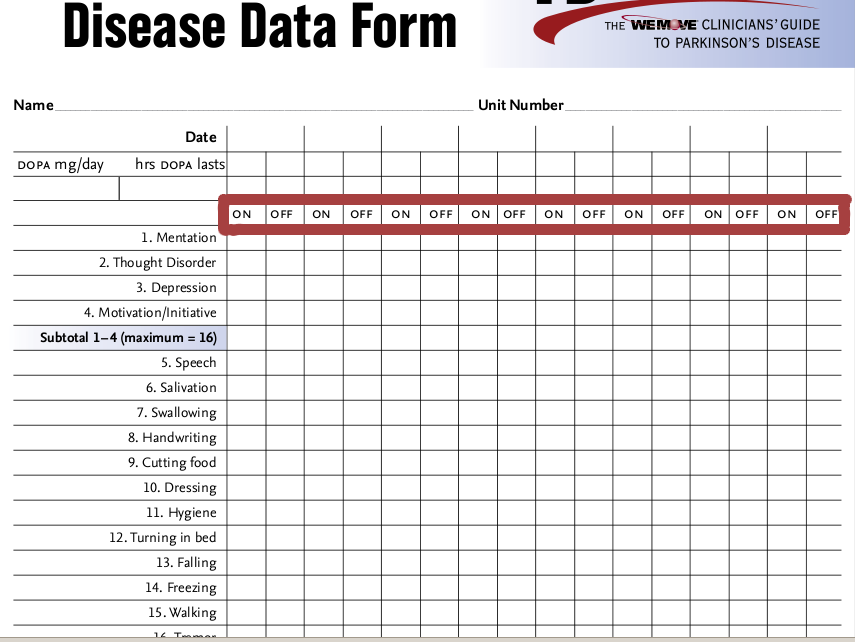
\includegraphics[height=2.4 in]{img/updr1-sel.png}
    \end{block}		
\end{frame}

% \begin{frame}{Escala (UPDRS)} 
%     \begin{block}{Impacto nas Atividades Diárias}
%       \center 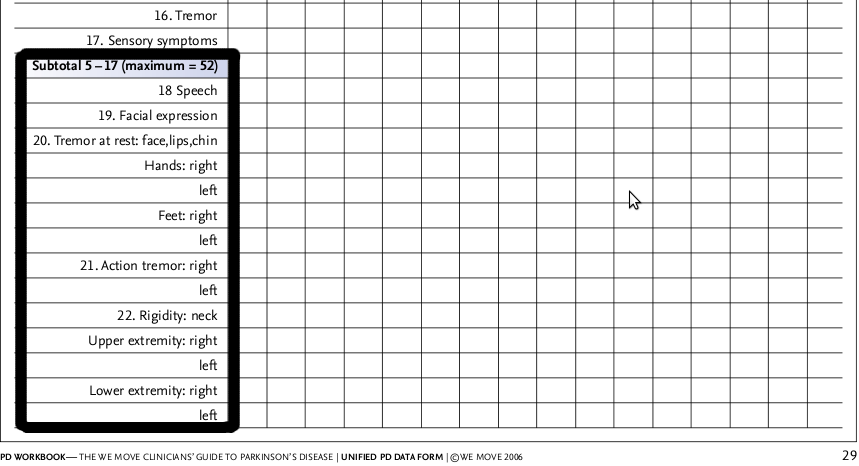
\includegraphics[height=2.0 in]{img/updr2-sel.png}
%     \end{block}
% \end{frame}


\subsection{Entrevista}
\begin{frame}{Entrevista Semi-Estruturada com Profissionais de Saúde} 
    \begin{block}{Objetivo da Pesquisa}
    O objetivo da entrevista semiestruturada foi entender como é feito o acompanhamento do paciente com sintomatologia do Parkinson, juntamente aos profissionais de saúde.
    \end{block}
		\begin{block}{Participantes}
			\begin{table}[h]
			%\caption{Perfil dos Participantes}
			%\label{table:perfil_analise_participantes}
			\begin{tabular}{|l|l|c|c|}
			\hline
			\textbf{LEGENDA} & \textbf{PROFISSÃO}             & \multicolumn{1}{|l|}{\textbf{EXPERIÊNCIA (ANOS)}} \\ \hline
			FIS\_01          & Fisioterapeuta & 10                                                \\ \hline
			FIS\_02          & Fisioterapeuta    & 10                                                \\ \hline
			NEU\_01          & Neurologista            & 15                                                \\ \hline
			NEU\_02          & Neurologista            & 30                                                \\ \hline
			\end{tabular}
			\end{table}
    \end{block}
\end{frame} 

\begin{frame}{Resultado da Entrevista} 
    \begin{block}{}
			\begin{itemize}[<+->]
				\item Identificamos a importância de \textbf{monitorar a bradicinesia para acompanhar a evolução do Parkinson}.
				\item Os profissionais de saúde informaram da importância de calcular:
					\begin{enumerate}
						\item amplitude dos movimentos de abdução e adução dos braços;
						\item a velocidade angular desse movimento.
					\end{enumerate}
			\end{itemize}
    \end{block}
\end{frame} 

\section{Abordagem JOGUE-ME}
\subsection{Apresentação}
\begin{frame}{Abordagem JOGUE-ME}
    \begin{block}{}
    A abordagem \textbf{JOGUE-ME} faz uso de jogos eletrônicos como interface de aquisição de sinais, tornando os usuários mais motivados a fornecer seus dados motores, em comparação ao uso dos dispositivos vestíveis.
    \end{block}
    
    
    \begin{block}{}
    Este trabalho pretende usar um ambiente de jogo para a execução de movimentos específicos com o propósito de quantificar os sinais motores dos usuários e consequentemente realizar o monitoramento. 
    \end{block}
\end{frame}

\begin{frame}{Visão Geral da Abordagem~\textit{JOGUE-ME}}
  \begin{block}{}
      \center 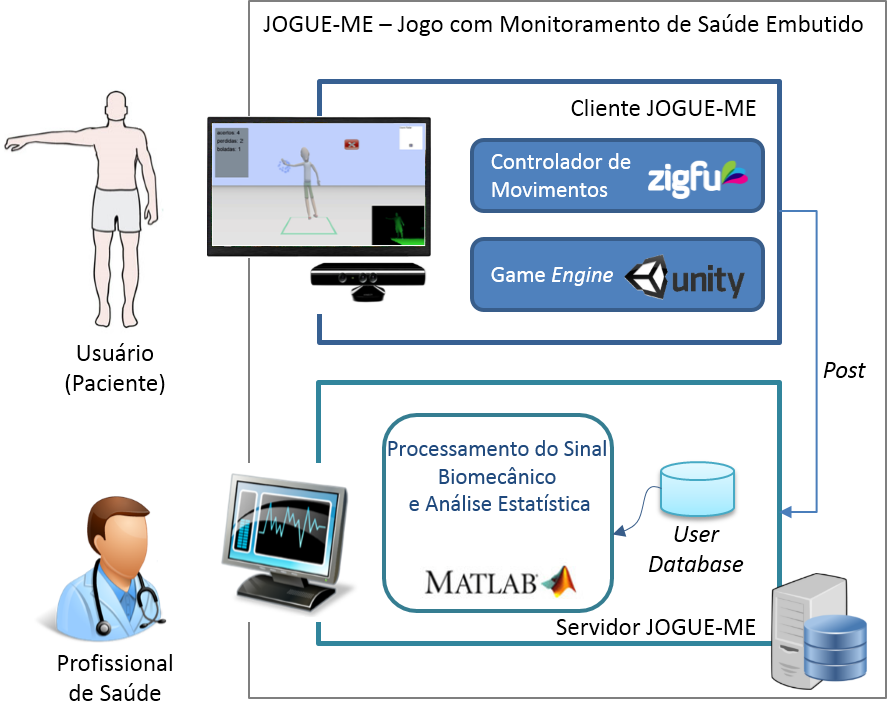
\includegraphics[height=1.8 in]{img/visaosistema.png}
  \end{block}
\end{frame}


\begin{frame}{JOGUE-ME - \textit{Jogo com Monitoramento de Saúde Embutido}}
	\begin{block}{}
		\begin{itemize}[<+->]
			\item	\textbf{REQ-JOGUE-ME-01} - Pontuação e Taxa de Acerto;
			\item	\textbf{REQ-JOGUE-ME-02} - Progresso e Evolução do Jogador e dos Desafios;
			\item	\textbf{REQ-JOGUE-ME-03} - Estado de Fluxo;
			\item	\textbf{REQ-JOGUE-ME-04} - Preocupação com Integridade Física do Jogador;
			\item	\textbf{REQ-JOGUE-ME-05} - Aquisição e Armazenamento de Sinais Motoress;
			\item	\textbf{REQ-JOGUE-ME-06} - Mecanismo de Identificação de Sintomas Motores;
			\item	\textbf{REQ-JOGUE-ME-07} - Mecanismo de Visualização.
		\end{itemize}
	\end{block}
\end{frame}

\subsection{Processamento de Sinais}
\begin{frame}{Processamento dos Sinais Biomecânicos}
  \begin{block}{}
      \center 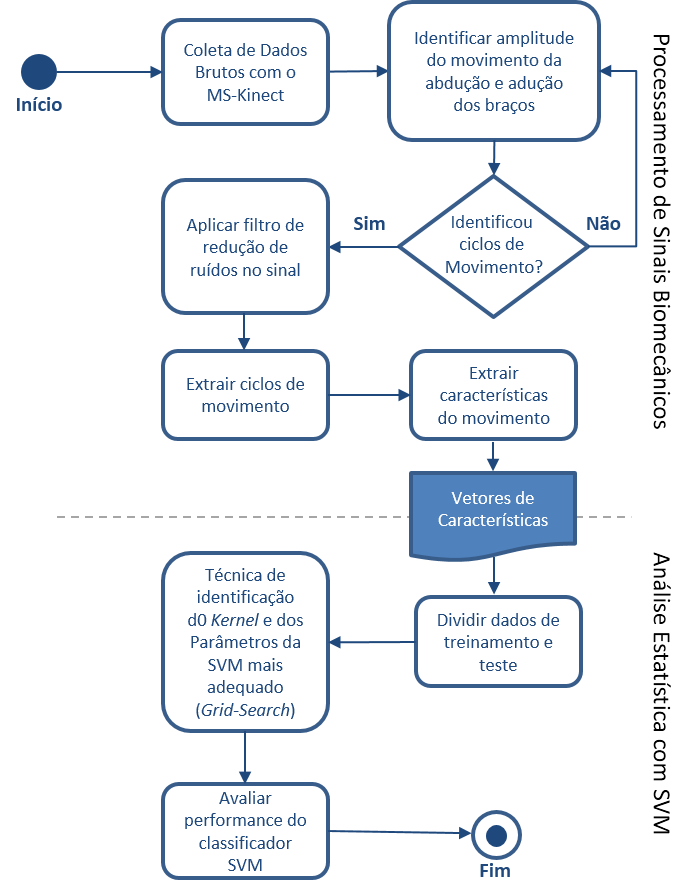
\includegraphics[height=2.4 in]{img/biomecprocessor2.png}
  \end{block}
\end{frame}


\begin{frame}{Cinemetria}
  \begin{block}{}
      \begin{itemize}[<+->]
	 \item A Cinemetria consiste de um conjunto de métodos para medir os valores dos parâmetros cinemáticos;
	 \item Movimento Cinético é o estudo das forças e momentos que resultam no movimento do corpo e seus segmentos.
       \end{itemize}
  \end{block}
\end{frame}


\begin{frame}{Sensor de Captura de Movimentos}
  \begin{block}{\textit{Ms-Kinnect 1.0} e os Pontos Selecionados}
      \center 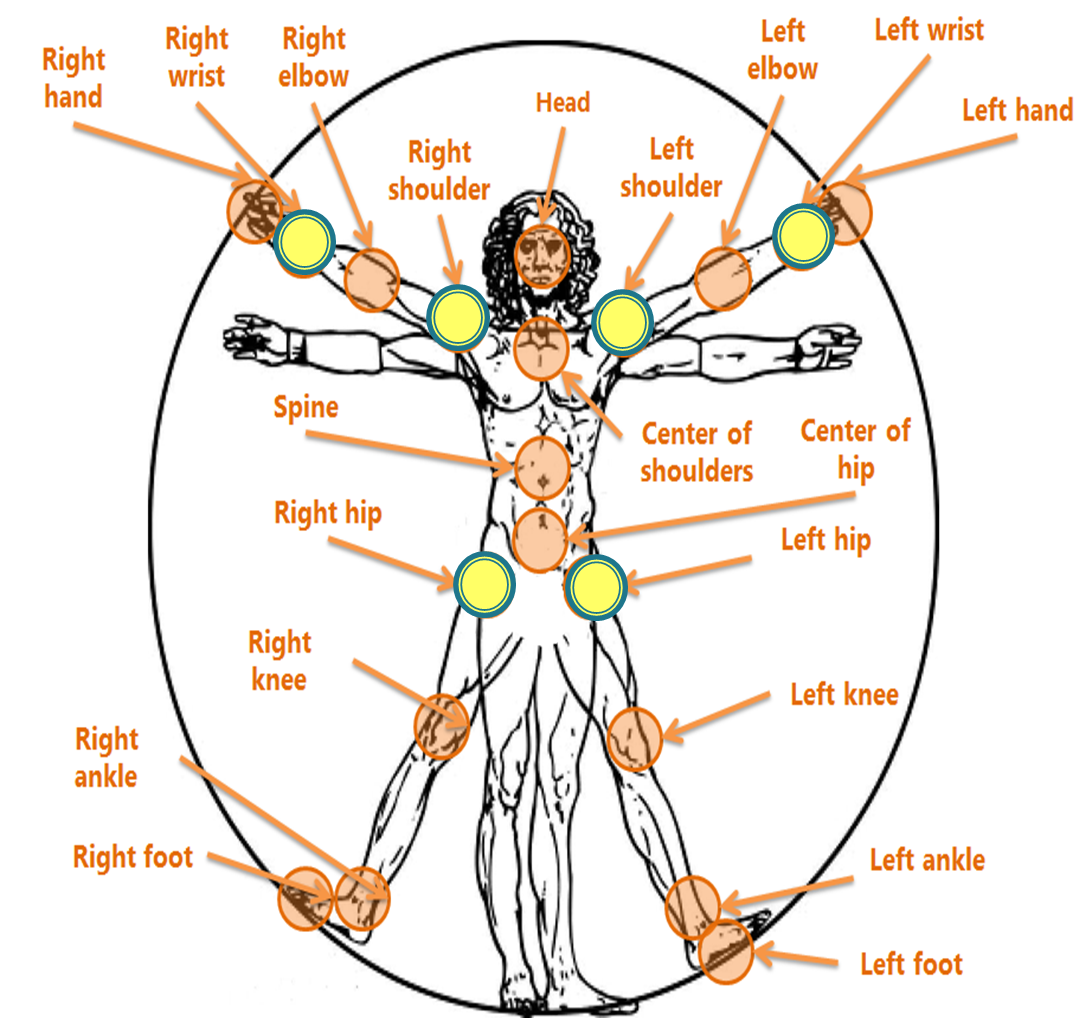
\includegraphics[height=2.5 in]{img/articulacoes-sel.png}
			%\caption{Modificações no Jogo ao Longo das Fases de Desenvolvimento~\cite{fullerton2008game}}
  \end{block}
\end{frame}

\begin{frame}{Movimento Angular}
  \begin{block}{Movimento de Abdução e Adução do Braço ~\cite{mcginnis2013biomechanics}}
      \center 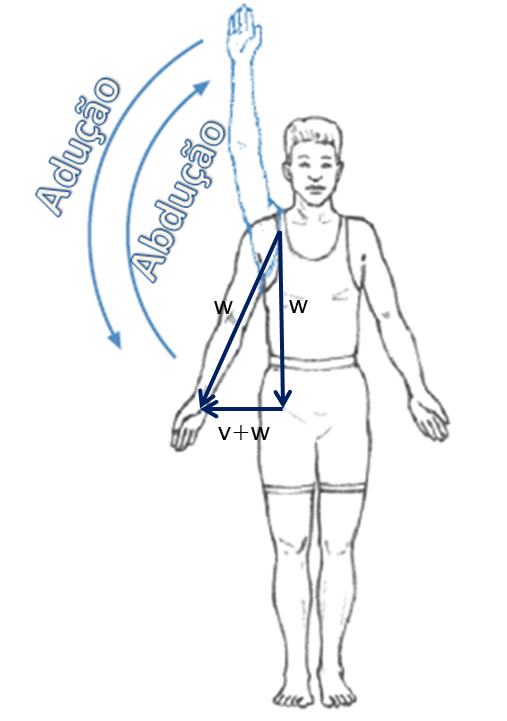
\includegraphics[width=4cm]{img/abducao-angulo.png}
  \end{block}
\end{frame}

% \begin{frame}{Mecanismo de Identificação de Sintomas Motores}
%       \center 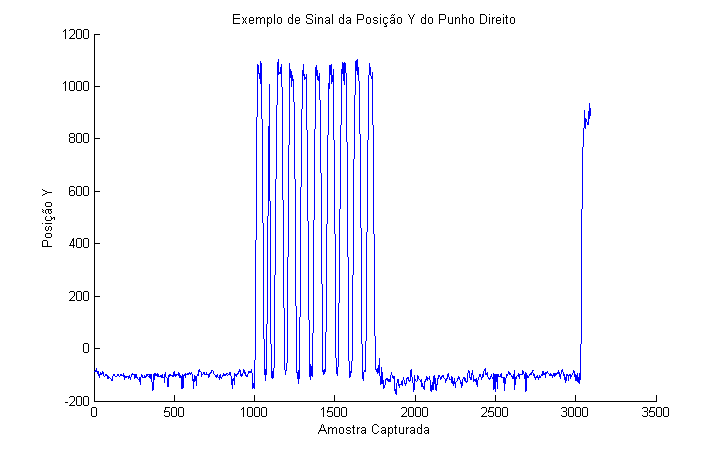
\includegraphics[height=3 in]{img/exsinalposicaoypunhodireito.png}
% \end{frame}

% \begin{frame}{Técnicas de Picos e Vales do Sinal}
%   \begin{block}
%       \center 
%       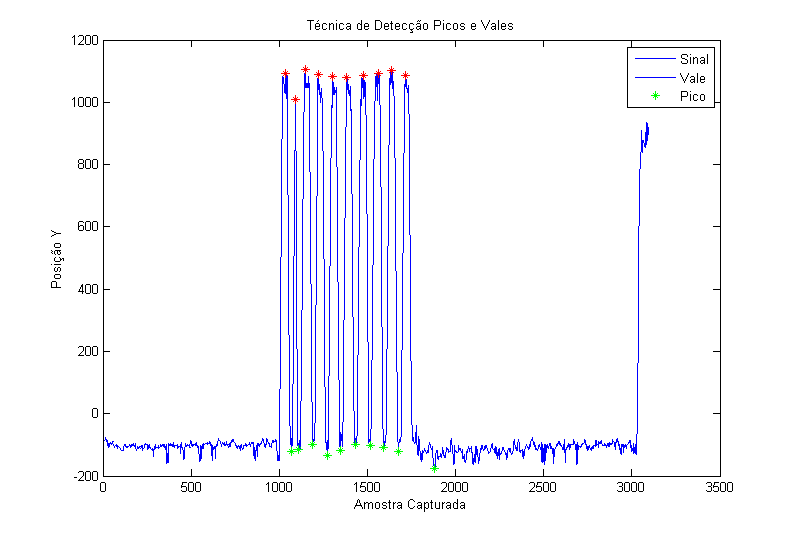
\includegraphics[height=2.8 in]{img/deteccaopicosvales.png}
%   \end{block}
% \end{frame}
% 
% 
% 

\begin{frame}{Mecanismo de Identificação de Sintomas Motores}
     \begin{block}{}
      \center 
      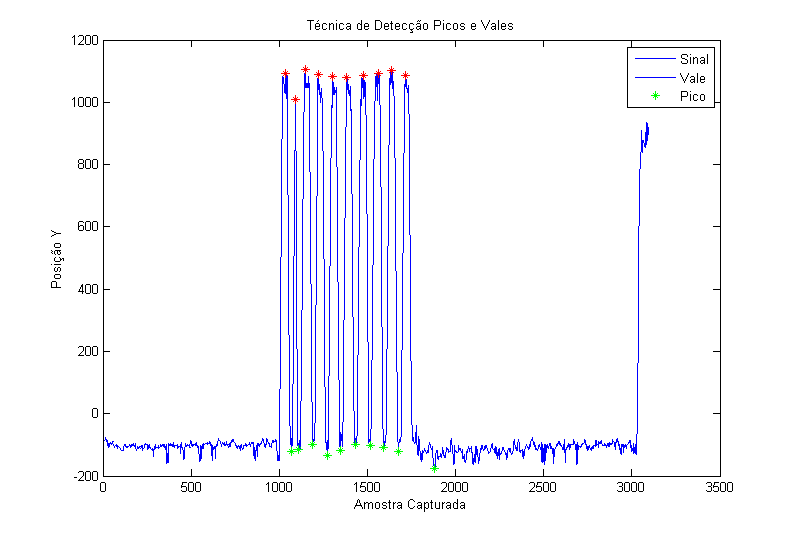
\includegraphics[height=2.2 in]{img/deteccaopicosvales.png}
			%\caption{Modificações no Jogo ao Longo das Fases de Desenvolvimento~\cite{fullerton2008game}}
     \end{block}
\end{frame}


\begin{frame}{Velocidade Angular do Movimento de Abdução e Adução}
     \begin{block}{}
      \center 
      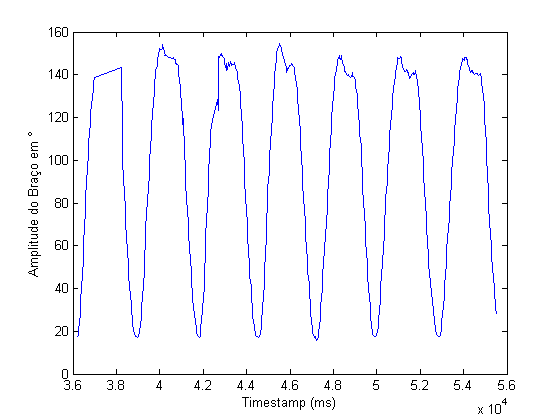
\includegraphics[height=2.2 in]{img/amplitude-braco.png}
			%\caption{Modificações no Jogo ao Longo das Fases de Desenvolvimento~\cite{fullerton2008game}}
     \end{block}
\end{frame}

\begin{frame}{Filtragem de Dados: Remoção de Ciclos Incompletos}
   \begin{block}{}
   
   \begin{columns}[c]
     \begin{column}{0.5\linewidth}
				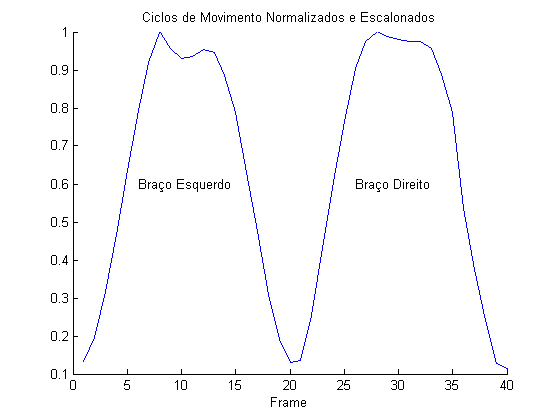
\includegraphics[width=5.5cm]{img/ciclonormalizadoescalonado.png}
     \end{column}

     \begin{column}{0.55\linewidth}
				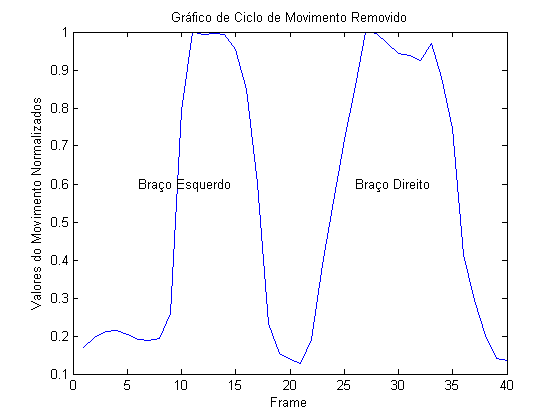
\includegraphics[width=5.5cm]{img/ciclomovimentoremovido.png}
    \end{column}
\end{columns}
\end{block}
\end{frame}

\subsection{Classificador de Dados}
\begin{frame}{Classificador de Dados}
\begin{block}{}
			O classificador de dados, é utilizado para identificar possíveis usuários com problemas motores. 			
			
\end{block}
\end{frame}

\begin{frame}{Máquina de Vetor de Suporte (SVM)}
   \begin{block}{}
   
   \begin{columns}[c]
     \begin{column}{0.5\linewidth}
			 \begin{itemize}
				\item Uma SVM utiliza vetores de separação através de uma técnica de hiperplano de separação ótima.

				\item Formalmente, classificadores que separam os dados por meio de um hiperplano utilizam um discriminante linear~\ref{eq:hiperplano}.
			\end{itemize}

			\begin{equation}
			f(x)=w^Tx+b
			\label{eq:hiperplano}
			\end{equation}.
     \end{column}

     \begin{column}{0.5\linewidth}
				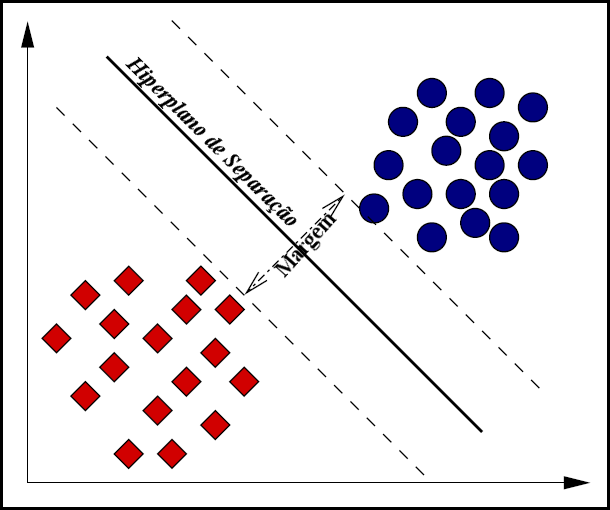
\includegraphics[width=4cm]{img/svmhyperplane.png}
    \end{column}
\end{columns}
\end{block}
\end{frame}

% \begin{frame}{Visualização do Vetor Médio do Movimento de Abdução e Adução do Braço}
%       \center 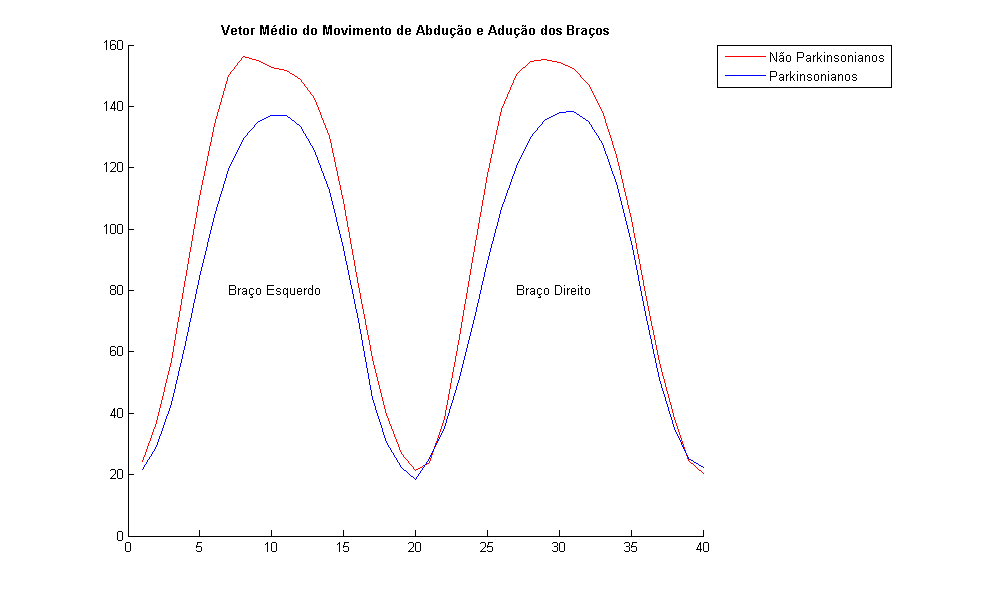
\includegraphics[height=2.6 in]{img/vetormedioaducao.png}
% \end{frame}

% \begin{frame}{Ciclos de Movimento de Abdução e Adução do Braço}
%       \center 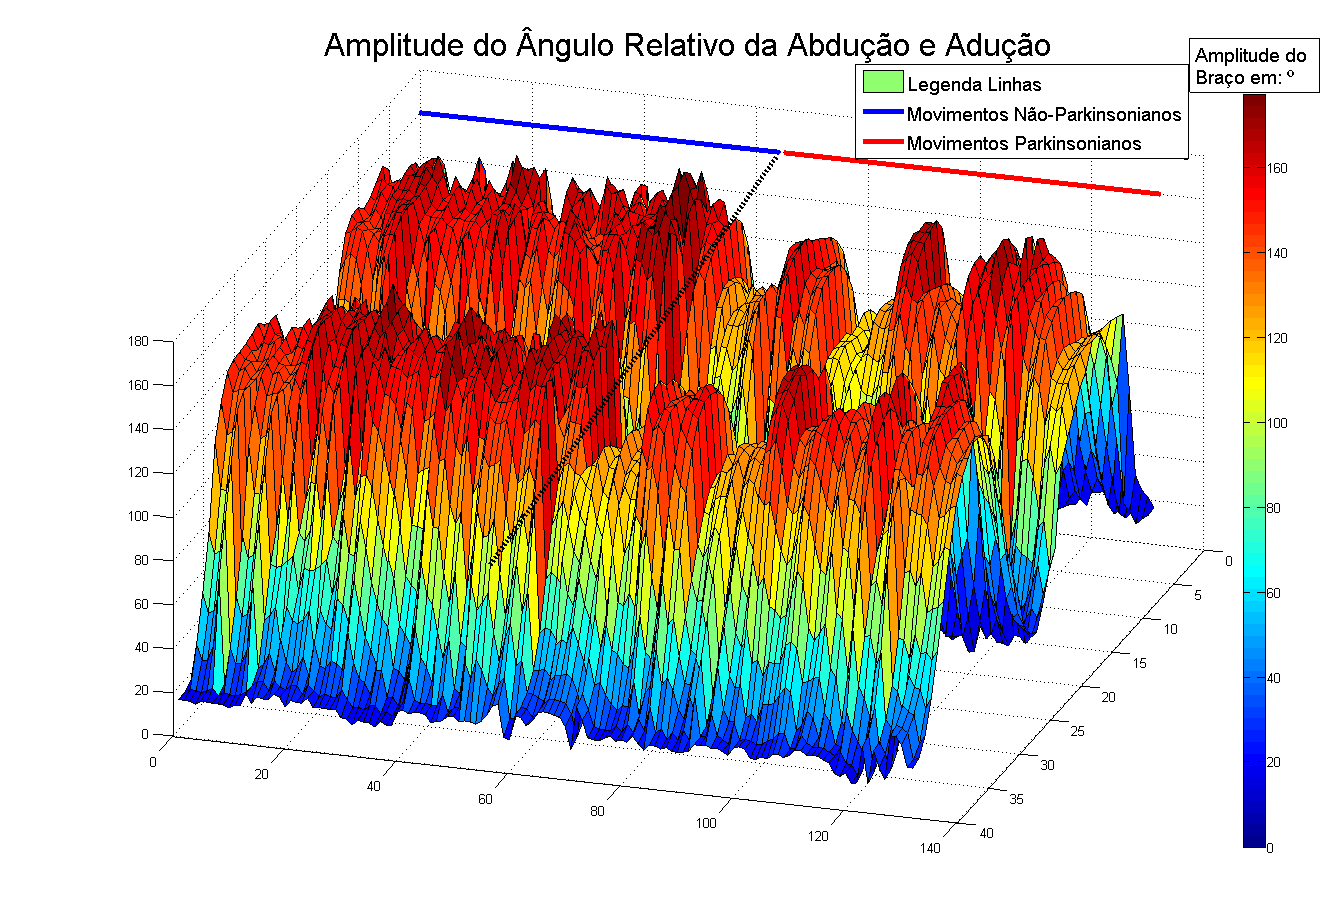
\includegraphics[height=3 in]{img/ciclosmovimentokinnect-2.png}
% \end{frame}


% \begin{frame}{Visualização das Características do Movimento}
%   \begin{block}{}
%       \center 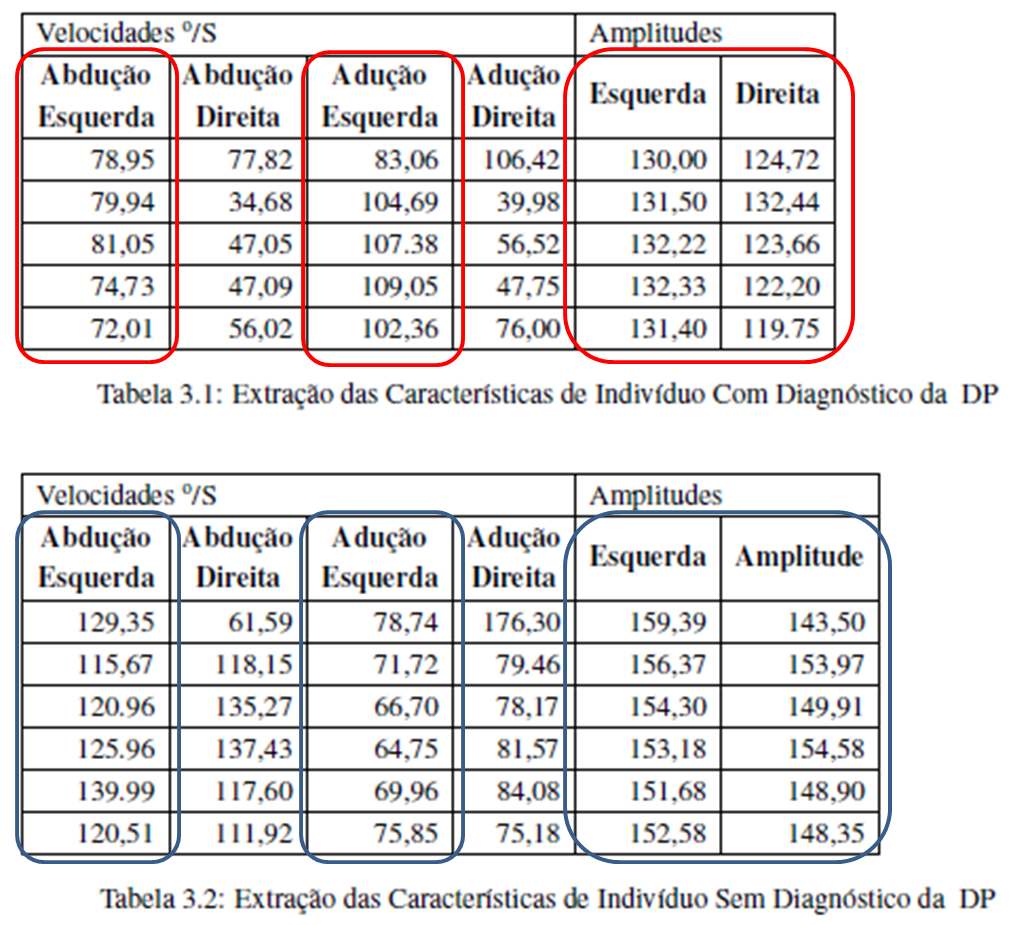
\includegraphics[height=2.6 in]{img/caracteristicas-tabela.png}
%   \end{block}
% \end{frame}

\section{Experimentos}
\subsection{Caso-Controle}
%\subsection{Estudo Analítico de Caso-Controle}
\begin{frame}{Estudo Analítico de Caso-Controle: Identificação da Bradicinesia} 
    \begin{block}{Objetivo da Pesquisa}<1->

    
    Como melhor adquirir e quantificar sinais motores utilizando sensores de movimento para monitorar os sinais do Parkinson?

    \end{block}
		\begin{block}{Coleta de Dados}<2->
			\begin{itemize}
				\item Protocolo de pesquisa submetido aprovado junto ao CEP da UFCG (\textbf{CAAE: 14408213.9.1001.5182})
				\item Coleta realizada nas instituições:
					\begin{enumerate}
						\item Hospital Universitário da UFAL;
						\item Fundação Pestalozzi;
						\item Clínica Fisioterapia do CESMAC.
				\end{enumerate}				
			\end{itemize}
    \end{block}
\end{frame}

\begin{frame}{Amostra} 
    \begin{block}{}
			\begin{itemize}[<+->]
				\item A técnica de amostragem utilizada para seleção, foi por conveniência, composta por:
				\begin{enumerate}
					\item 15 indivíduos portadores do Parkinson entre 51 e 65 anos (média de idade : 58 anos);
					\item 15 sem o diagnostico, como grupo controle entre 50 e 65 anos (média : 57 anos).
				\end{enumerate}
					\item No grupo de portadores do Parkinson, foram inclusos indivíduos até o Estágio 3 (Doença bilateral leve a moderada com alguma instabilidade postural e capacidade para viver independente), segundo a UPDRS.
				\end{itemize}
    \end{block}
\end{frame}
 
\begin{frame}{Coleta dos Dados Utilizando o Jogo: \textit{Catch the Spheres}}
      \center 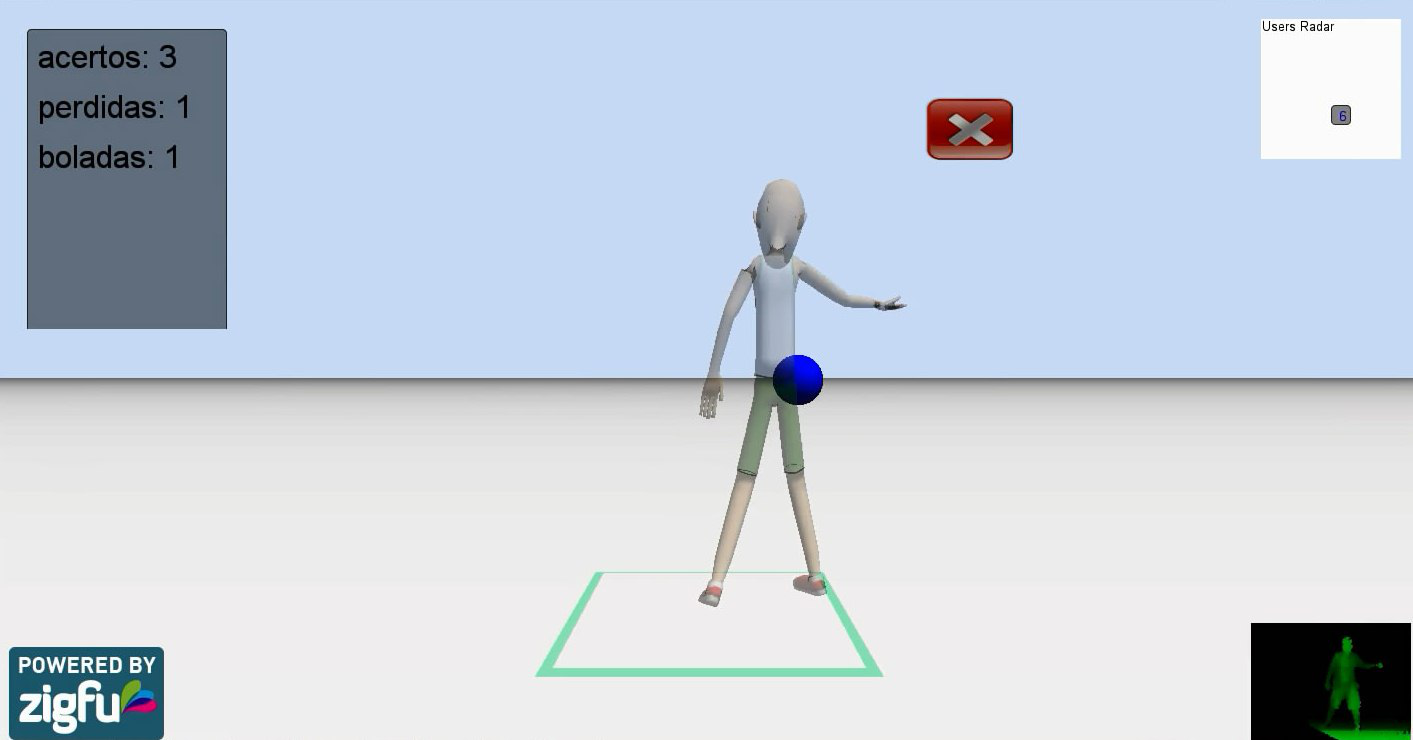
\includegraphics[height=2.2 in]{img/catch-the-spheres.png}
\end{frame}


\begin{frame}{Processo de Coleta de Dados}
   \begin{block}{}   
   \begin{columns}[c]
     \begin{column}{0.5\linewidth}
				\begin{itemize}[<+->]
					\item Voluntário se posiciona a 2m. do sensor de movimento;
					\item Voluntário inicia o jogo;
					\item Voluntário abduz e aduz o braço esquerdo, e depois o direito 10 vezes o mais amplo e rápido possível;
					\item Voluntário fecha o jogo.
				\end{itemize}
     \end{column}

     \begin{column}{0.55\linewidth}
				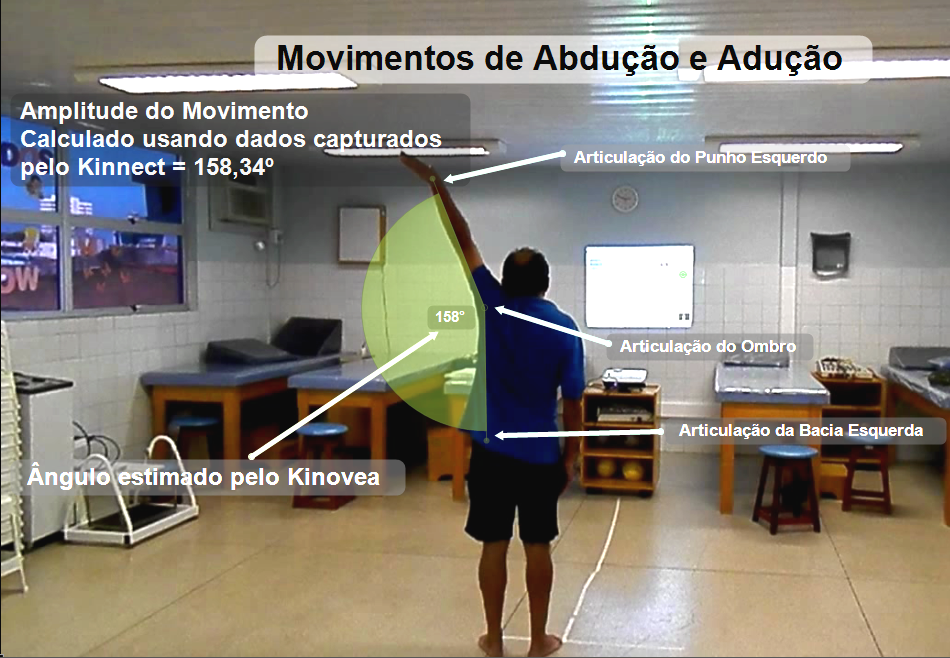
\includegraphics[width=5.5cm]{img/capturaducaokinnect.png}
    \end{column}
\end{columns}
\end{block}
\end{frame}
% 
% 
% 
% \begin{frame}{Processo de Coleta de Dados}
%   %\begin{block}{}
%       \center 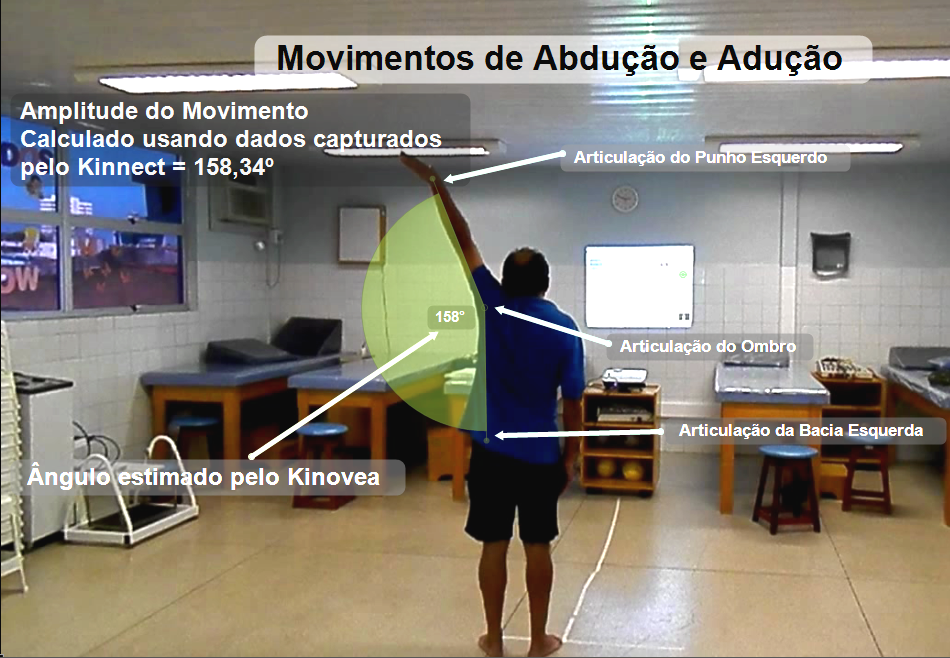
\includegraphics[height=2.6 in]{img/capturaducaokinnect.png}
% \end{frame}

% \begin{frame}{Características Extraídas do Movimento}
% 	\begin{block}{Descrição do vetor de características extraído da coleta de dados}
% 	\begin{table}[h]
% 	  \begin{tabular}{|l|l|}
% 	  \hline
% 	  {\bf Característica}  & {\bf Descrição}                                       \\ \hline
% 	  MaxAmpEsquerdo     & Amp. máxima do braço esquerdo. \\ \hline
% 	  MaxAmpDireito    & Amp. máxima do braço direito. \\ \hline
% 	  AngVelAbdEsquerdo  & Vel. ang. abdução do braço esquerdo. \\ \hline
% 	  AngVelAbdDireito & Vel. ang. da abdução do braço direito. \\ \hline
% 	  AngVelAdEsquerdo  & Vel. ang. da adução do braço esquerdo. \\ \hline
% 	  AngVelAdDireito & Vel. ang. de adução do braço direito. \\ \hline
% 	  \end{tabular}
% 	  \end{table}
% 
% 	
% % 		\begin{itemize}[<+->]
% % 			\item	Ciclo de movimento, normalizado e escalonado em 20 amostras;
% % 			\item	amplitude do movimento de abdução do braço esquerdo e direito;
% % 			\item	velocidade angular de abdução dos braços esquerdo e direito;
% % 			\item velocidade angular de adução do braço esquerdo e direito.
% % 		\end{itemize}
% 	\end{block}
% \end{frame}

\subsection{Classificação dos Dados}
\begin{frame}{Classificação dos Dados}
	\begin{block}{}
		\begin{itemize}[<+->]
			\item	Com os dados coletados, realizou-se uma classificação usando SVM com núcleo linear e \textit{bias} de 0,10.
			\item	O resultado com o núcleo linear foi o mais expressivo ante o Polinomial, Radial e MLP.
		\end{itemize}
	\end{block}
\end{frame}

\begin{frame}{Definição dos Parâmetros}
 \begin{block}{Aplicação do Método de \textit{Grid-Search}}
 Para identificar os melhores parâmetros da SVM, foi aplicado o método~\textit{Grid-Search} ~\cite{gridsearchsvm2010} usando validação cruzada \textit{Leave-One-Out} (LOOCV)~\cite{kantardzic2011data}.   
 \end{block}
\end{frame}

% \begin{frame}{Definição dos Parâmetros}
%  \begin{block}{Parâmetros utilizados no \textit{Grid-Search}}
%     Os valores dos parâmetros de pesquisa do \textit{grid-search} foram de: $C$ = [$2^5$, ... ,$2^2$] e $\gamma$ = [$2^{15}$, ... ,$2^3$ ], usando assim uma exponencial de base 2. Por meio deste método, foi possível identificar uma região em que o classificador possuía a melhor acurácia e a menor taxa de \textit{FpRate}. Após identificar essa região, realizamos uma busca mais detalhada com os seguintes parâmetros: $C$ = [0.25, 0.5, ... ,2.5]; e $\gamma$ = [1, 2, ...,10].
%  \end{block}
% \end{frame}

\begin{frame}{\textit{Grid-Search} - Acurácia da Classificação}
  \begin{block}{}
  \center  
  %\begin{block}{}
      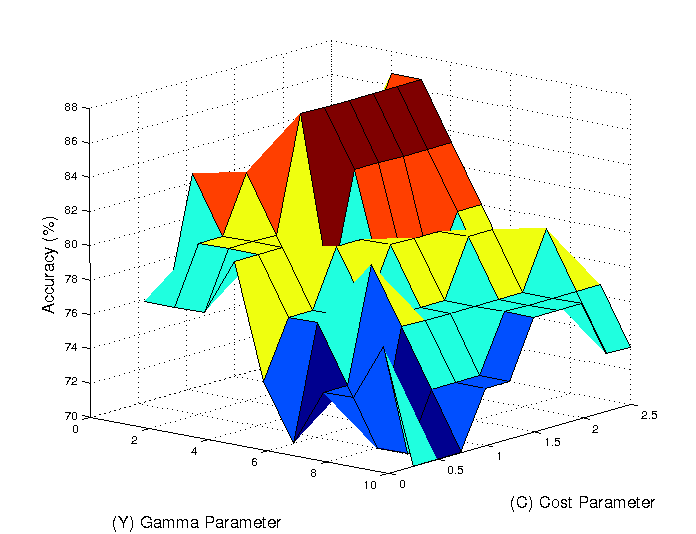
\includegraphics[scale=0.4]{./img/gridsearch.png}      
  \end{block}
\end{frame}

\begin{frame}{\textit{Grid-Search} - \textit{FpRate}}
   \begin{block}{}
   \center
  %\begin{block}{}
      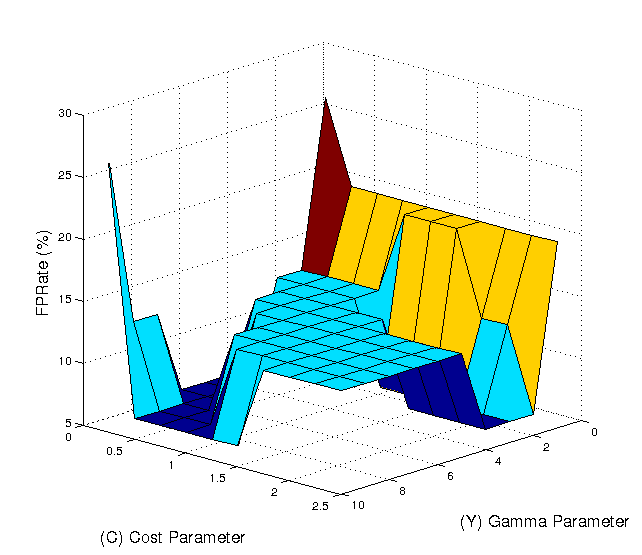
\includegraphics[scale=0.4]{./img/gridsearchfprate.png}
   \end{block}
\end{frame}

\begin{frame}{Matriz de Confusão}
	\begin{block}{Resultado da Matriz de Confusão do Estudo Analítico Caso-Controle Usando SVM Linear}
\begin{table}[!htbp]
		\label{table:resultadomatrizconfusaosvm}
		\centering
		\begin{tabular}{l|c|c|}
		\cline{2-3}
		\multicolumn{1}{c}{}                         & \multicolumn{2}{|c|}{\textit{\textbf{Classe Preditiva}}} \\ \cline{2-3} 
																								 & \textbf{Parkinson}      & \textbf{Controle}         \\ \hline
		\multicolumn{1}{|l|}{\textbf{Parkinson}} & 12       & 3           \\ \hline
		\multicolumn{1}{|l|}{\textbf{Controle}}     & 1           & 14     \\ \hline
		\end{tabular}
\end{table}
	\end{block}
\end{frame}

\begin{frame}
   \frametitle{Métricas da Classificação}
   \begin{block}{}
   		\begin{table}[!htbp]
				\label{table:metricasmatrizconfusao}
				\centering
				\begin{tabular}{|l|r|}
				\hline
				\multicolumn{2}{|l|}{\textbf{Métricas}} \\ \hline
				\textbf{TpRate}                    & 80,00$\%$\               \\ \hline
				\textbf{FpRate}                    & 6,67$\%$\                \\ \hline
				\textbf{Precision}                 & 92,31$\%$\                \\ \hline
				\textbf{Accuracy}                  & 86,67$\%$\                \\ \hline
				\textbf{F-Measure}                 & 85,71$\%$\                \\ \hline
				\end{tabular}
				\end{table}
	\end{block}
     \begin{block}{}
				\begin{description}
				\item [\textit{TpRate}]: taxa de acerto obtido;
				\item [\textit{FpRate}]: taxa de falso alarme obtido;
				\item [\textit{Precision}]: taxa de acerto de uma instância em determinada classe;
				\item [\textit{Accuracy}]: taxa de acerto de todo o classificador;
				\item [\textit{F-Measure}]: análise de classificador binário que mede a acurácia.
				\end{description}
    \end{block}
\end{frame}

\subsection{Limitações}
\begin{frame}{Limitações do Método}
	\begin{block}{}
	A aprendizagem estatística deste trabalho é apenas um indicador e necessita da interpretação do profissional de saúde.
	\end{block}
  \begin{block}{}
      \center 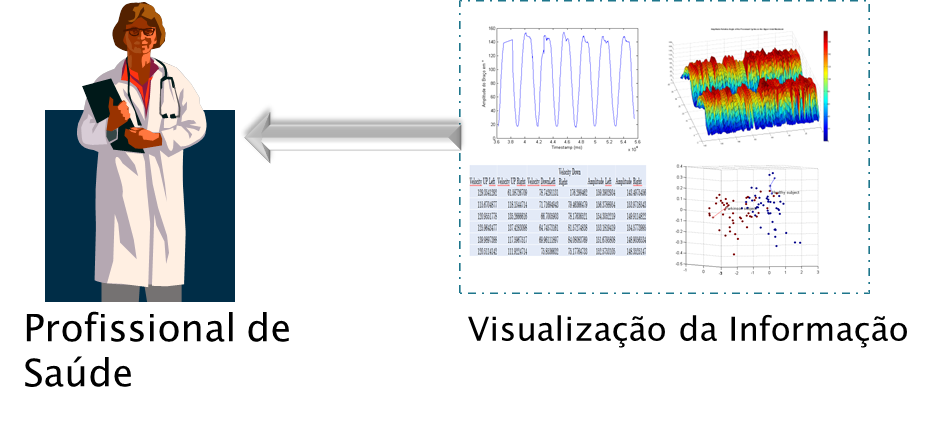
\includegraphics[height=1.6 in]{img/visualizacaomedico.png}
  \end{block}
\end{frame}

\begin{frame}{Outros Experimentos}
	\begin{block}{Uso de Jogo em \textit{Smartphone} Para Detecção de Tremor}
	\center 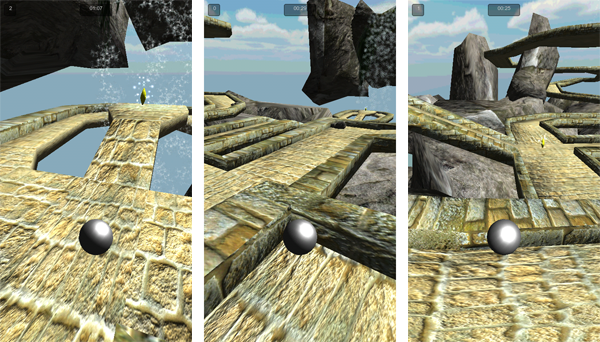
\includegraphics[height=1 in]{img/pinball_world.png}
	\end{block}
	\begin{block}{Insucesso na Quantificação do Tremor}
			\begin{itemize}[<+->]
			\item Tremor do Parkinson é de repouso;
			\item Indivíduos quando utilizavam o jogo reduziam drasticamente o sintoma;
			\item Como os dados não seriam satisfatórios, logo a coleta tornou-se inviável.
		\end{itemize}
	\end{block}
\end{frame}






\section{GQM}
\subsection{Análise}
\begin{frame}{Análise GQM com Usuários} 
    \begin{block}{Objetivo da Pesquisa}
      Etapa 3 da Pesquisa: Na perspectiva dos usuários, a abordagem de quantificar os sinais motores é considerada não-invasiva e aplicável à rotina diária?
    \end{block}
		\begin{block}{Participantes}
		Nessa etapa da pesquisa foram avaliados 30 sujeitos, dos seguintes locais: 
			\begin{itemize}
				\item Hospital Universitário da UFAL;
				\item Fundação Pestalozzi;
				\item Clínica de Fisioterapia do CESMAC.
			\end{itemize}
    \end{block}
\end{frame} 


\begin{frame}{Questões da Pesquisa} 
    \begin{block}{}
			\begin{enumerate}
				\item O usuário poderia integrar a abordagem JOGUE-ME à sua rotina diária ?
				\item A segurança com a integridade física está de acordo com a faixa etária do usuário ?
			\end{enumerate}
    \end{block}
\end{frame}


%  \begin{table}[h]
%   \begin{tabular}{|p{10cm}|p{1.2cm}|p{1.2cm}|}
%   \hline
%   \textbf{Métrica} & \textbf{Sim} & \textbf{Não} \\ \hline
%   1.2: O jogo traz motivação ao usuário? & 91,67\% & 8,33\% \\ \hline
%   1.4: O usuário considera o jogo simples, sem muitas regras e de fácil entendimento? Ele pode ser aplicado em diferentes idades? & 91,67\% & 8,33\% \\ \hline
%   1.5: O usuário tem o costume de jogar esses jogos casuais em casa? & 41,67\% & 58,33\% \\ \hline
%   1.6: O usuário agregaria um jogo desse estilo em sua rotina diária? & 75\% & 25\% \\ \hline
%   2.1: Uma criança estaria segura jogando esse jogo, ao efetuar os movimentos dos braços? & 100\% & 0\% \\ \hline
%   2.2: Um adulto estaria seguro ao jogar esse jogo, ao efetuar os movimentos dos braços? & 100\% & 0\% \\ \hline
%   2.3: Um idoso estaria seguro ao jogar esse jogo, ao efetuar os movimentos dos braços? & 75\% & 25\% \\ \hline
%   \end{tabular}
%   \end{table}

% \begin{frame}{Métricas Avaliadas do \textit{GQM}} 
%   \begin{block}{Questão 1: Integração à Rotina Diária}
%     \begin{table}[h]
%   \begin{tabular}{|p{8cm}|p{1.2cm}|p{1.2cm}|}
%   \hline
%   \textbf{Métrica} & \textbf{Sim} & \textbf{Não} \\ \hline
%   1.2: O jogo traz motivação ao usuário? & 91,67\% & 8,33\% \\ \hline
%   1.4: O usuário considera o jogo simples, sem muitas regras e de fácil entendimento? Ele pode ser aplicado em diferentes idades? & 91,67\% & 8,33\% \\ \hline
%   1.5: O usuário tem o costume de jogar esses jogos casuais em casa? & 41,67\% & 58,33\% \\ \hline
%   1.6: O usuário agregaria um jogo desse estilo em sua rotina diária? & 75\% & 25\% \\ \hline
%   \end{tabular}
%   \end{table}
%   \end{block} 
% \end{frame}
% 
% \begin{frame}{Métricas Avaliadas do \textit{GQM}} 
%   \begin{block}{Questão 2: Segurança e Integridade Física}
%     \begin{table}[h]
%   \begin{tabular}{|p{8cm}|p{1.2cm}|p{1.2cm}|}
%   \hline
%   \textbf{Métrica} & \textbf{Sim} & \textbf{Não} \\ \hline
%   2.1: Uma criança estaria segura jogando esse jogo, ao efetuar os movimentos dos braços? & 100\% & 0\% \\ \hline
%   2.2: Um adulto estaria seguro ao jogar esse jogo, ao efetuar os movimentos dos braços? & 100\% & 0\% \\ \hline
%   2.3: Um idoso estaria seguro ao jogar esse jogo, ao efetuar os movimentos dos braços? & 75\% & 25\% \\ \hline
%   \end{tabular}
%   \end{table}
%   \end{block} 
% \end{frame}

\begin{frame}{Integrar a Abordagem à Rotina Diária} 
    \begin{block}{Métrica 1.1: Escala de Diversão do Jogo}
			\center 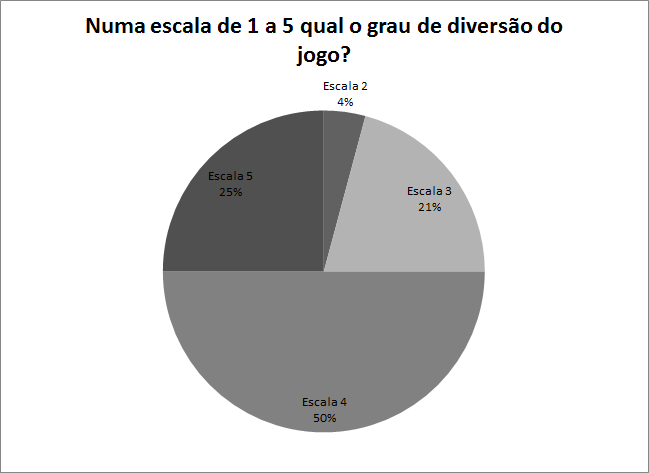
\includegraphics[height=2.4 in]{img/chart_1-.png}
    \end{block}
\end{frame}

\begin{frame}{Integrar a Abordagem à Rotina Diária} 
    \begin{block}{Métrica 1.3: Integrar o Jogo À Rotina Diária}
			\center 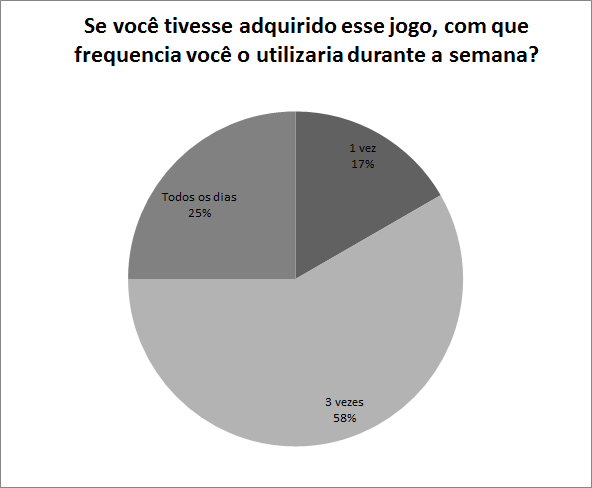
\includegraphics[height=2.4 in]{img/chart_3-.png}
    \end{block}
\end{frame}

\begin{frame}{Integrar a Abordagem à Rotina Diária} 
    \begin{block}{}
			\center 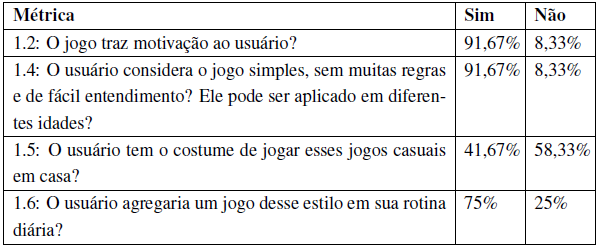
\includegraphics[height=1.4 in]{img/metricasq1.png}
    \end{block}
\end{frame}

\begin{frame}{Segurança à Integridade Física} 
    \begin{block}{Métrica 2.4: Faixa Etária do Jogo}
			\center 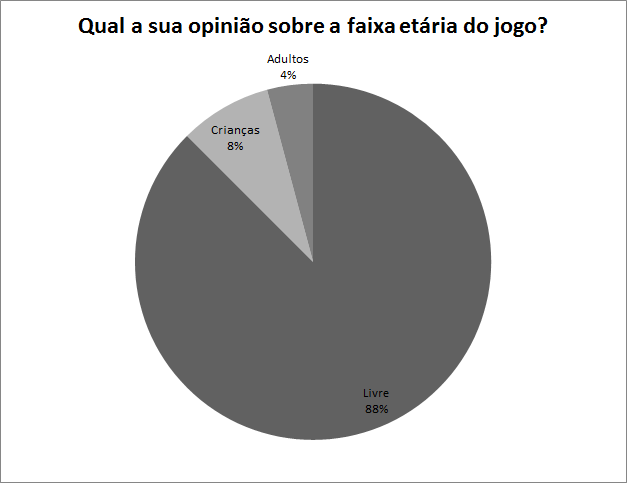
\includegraphics[height=2.4 in]{img/chart_10-.png}
    \end{block}
\end{frame}

\begin{frame}{Segurança à Integridade Física} 
    \begin{block}{}
			\center 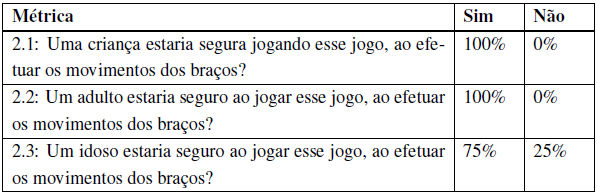
\includegraphics[height=1.4 in]{img/metricasq2.png}
    \end{block}
\end{frame}


\section{Finalização}
\subsection{Conclusão e Trabalhos Futuros}

\begin{frame}{Conclusão}
\begin{block}{}
Nos experimentos realizados, conseguimos demonstrar:
  \begin{itemize}[<+->]
   \item A importância do acompanhamento dos sinais motores integrados à rotina diária do paciente;
   \item A viabilidade do desenvolvimento de jogos para o monitoramento, pois, obtivemos uma taxa de acurácia de 86,67\% e falsos positivos de 6,67\%;
   \item Um percentual de 83\% dos usuários integrariam a solução de monitoramento proposta em sua rotina diária.
  \end{itemize}
\end{block}
\end{frame}




\begin{frame}{Trabalhos Futuros}
\begin{block}{}
A partir dos resultados apresentados nesta tese e extensão da mesma, alguns trabalhos futuros são propostos para contribuição científica:
  \begin{itemize}[<+->]
   \item Coletar uma amostra maior de pacientes com Parkinson, e agrupá-los de acordo com o estágio da doença~\cite{goul05};
   \item Usar técnicas de multi-classificação de dados~\cite{multisvm2011} para identificar o progresso do~\ac{dp} de acordo com as escalas de avaliação;
   \item Avaliar o sinal da bradicinesia em diferentes momentos do dia, para verificar a eficácia do tratamento medicamentoso~\cite{protpar010}.   
  \end{itemize}
\end{block}
\end{frame}


\subsection{Publicações}
\begin{frame}{Publicações}
\begin{block}{}
Foram publicados três artigos, em conferências internacionais, relacionados à tese: 
  \begin{itemize}
   \item \textit{Abstract}: \textit{Monitoring Parkinson related Gait Disorders with Eigengaits}, no, \textit{XX World Congress on Parkinson's Disease and Related Disorders} (2013)~\cite{lmmeigengaits2013};
   \item \textit{Full Paper}: \textit{A Game-Based Approach to Monitor Parkinson’s Disease: The bradykinesia symptom classification}, no, \textit{International Symposium on Computer-Based Medical Systems} (CBMS 2016)~\cite{lmmcbmsgame2016};
   \item \textit{Full Paper}: \textit{A Gait Analysis Approach to Track Parkinson’s Disease Evolution Using Principal Component Analysis}, no, \textit{International Symposium on Computer-Based Medical Systems} (CBMS 2016)~\cite{lmmcbmsgait2016}.
  \end{itemize}
\end{block}
\end{frame}

\subsection{Dúvidas}
\begin{frame}
  \begin{center}
  DÚVIDAS ?
  \end{center}
\end{frame}

\bibliographystyle{authordate2}
\bibliography{biblmmcor} % arquivos com as entradas bib.

\end{document}
	